\chapter{Transport og reise}

\section{Fly}
SAS og Norwegian flyr fra flere store byer i Tyskland. Bestiller man i god tid, kan man få billetter til og fra München til under tusenlappen.
Hvis man er litt sent ute og flybilletten til Norwegian er litt dyr kan man sjekke SAS sine ungdomsbilletter, der får man også bagasje inkludert. 

\url{http://www.sas.no/}

Eller bruk finn.no sine sider og søk opp de billigeste billettene til de dagene en ønsker å reise. 

\url{http://www.finn.no/finn/travel/air/search}

Hvis du skal til andre byer enn Oslo, har KLM som oftest de beste tilbudene. Det kan svare seg å kjøpe enveisbillet til Tyskland, for så å reise tur/retur Tyskland, da det ofte biser seg at man får oppgitt bedre priser på nettet. Altså: Billetter kjøpt i Tyskland (Tyskland - Norge) er billigere enn billetter kjøpt i Norge (Norge - Tyskland).



\section{Tog}
Togsystemet i Tyskland er veldig pålitelig og effektivt, men også ganske dyrt. Hvis man har tenkt å benytte seg av togene, er det veldig lurt å kjøpe et BahnCard. Det finnes to typer; BahnCard25 og BahnCard50. Har man BC25 får man 25\% rabatt på alle reiser og med BC50 reiser man altså for halv pris. Disse koster ca 60\euro{} (BC25) og ca 120\euro{} (BC50) for et års bruk. Til sammenligning koster en togtur fra Frankfurt til Berlin uten BahnCard i underkant av 100\euro{}. Dvs at man skal ikke reise så veldig mye før det lønner seg med BahnCard. For mer info se \href{http://www.bahn.de}{www.bahn.de}.
Tog er kanskje ikke den billigste eller raskeste måten å komme seg til Norge fra München.


\section{Mitfahrgelegenheit}
Mitfahrgelegenheit er ganske populært her i Tyskland, organisert haiking. Kort forklart sitter man enkelt og greit på med noen som skal samme sted som deg. Under www.mitfahrgelegenheit.de kan man søke etter noen å sitte på med. Som oftest koster en tur rundt 10\euro{}, men av og til er det også gratis. Mange er litt skeptiske til denne "moderne haikingen", men det er faktisk veldig populært og trygt.

\url{http://www.mitfahrzentrale.de/} \\
\url{http://www.mitfahrgelegenheit.de/}


\begin{figure}[h]
\center
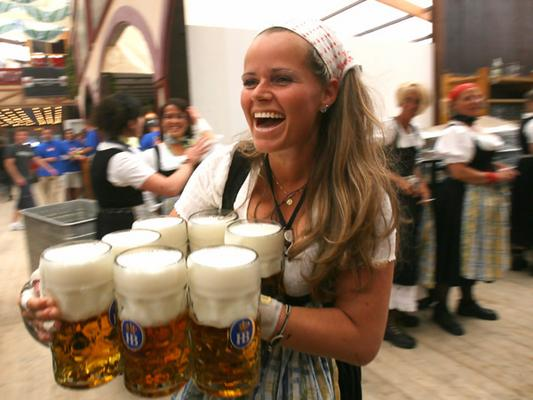
\includegraphics[width=0.31\textwidth]{./gfx/okt}
\caption{Bånn gass på oktoberfest}
\end{figure}

\section{Semesterticket}
Fra og med vintersemesteret 2013 tilbys det en semesterbillett for studenter i München. Se info her: \url{http://www.semesterticket-muenchen.de/}